\subsection{Controls and intermediate verification}
\label{sec:controls}

\textbf{The symbolic residual is an upper bound, and we tested it.} A residual against a solver may include
long-list handling rather than symmetry reasoning. Regressing per-structure $R_3$ correctness on
conventional-cell atom count over the same records (no new model calls): pooled over the 14 scored models
and 2940 model-structure pairs, Spearman $\rho = -0.0908$ at $p = 8.1\times10^{-7}$; 13 of 14 models are
negative, and accuracy falls from 0.5551 on cells at or below the median 14 atoms to 0.5129 above it
(Fisher $p = 0.0241$). The pre-registered confound control does not rescue it: atom count correlates with
crystal system ($\rho = -0.1866$), but the mean within-system association is $-0.1053$, stronger than the
pooled figure rather than attenuated, so the effect is not symmetry difficulty in disguise. We therefore
report the symbolic residual as an upper bound on a symmetry-reasoning deficit, not as a measurement of
one. Nothing here touches the oracle-to-model gap, which is measured against pixels.

\textbf{A learned extractor fabricates its output.} Substituting a strong model as the extraction stage,
prompted for species and positions with the symmetry question withheld, and having a weaker model answer
from that text yields 0.1429. That arm predicted two of seven classes and its accuracy equals the majority
stratum's base rate, so it measures nothing. The informative measurement is the intermediate, scored
directly against ground truth: median recall 0.0000, with 105 of 206 structures having not one emitted atom
within tolerance of a real one, despite a median of 48 well-formed atoms per structure. A colour-threshold
blob detector achieves median recall 0.400 on the same task. Downstream accuracy alone would have read this
as bad reasoning. \emph{A two-stage pipeline whose intermediate cannot be checked will attribute
fabrication to reasoning}, which is the argument for the instrument.

\textbf{The models do use the image.} A benchmark on which models score poorly invites the objection that
they are pattern-matching the prompt rather than reading the figure. We ran the image-absent control that
\citet{cotdeg2604} made standard: the identical prompt carrying the chemical formula and no renders. Every
scored model collapses toward seven-way chance (mean 0.1487), and the paired per-structure difference is
significant for 10 of the 13 models scored under the image-removal control (Figure~\ref{fig:noimage}); the
strongest model loses 0.5714. The three nulls are the three weakest models, two of which are not above
chance even with images, so those are floor effects rather than evidence of formula lookup.

\begin{figure}[t]
\centering
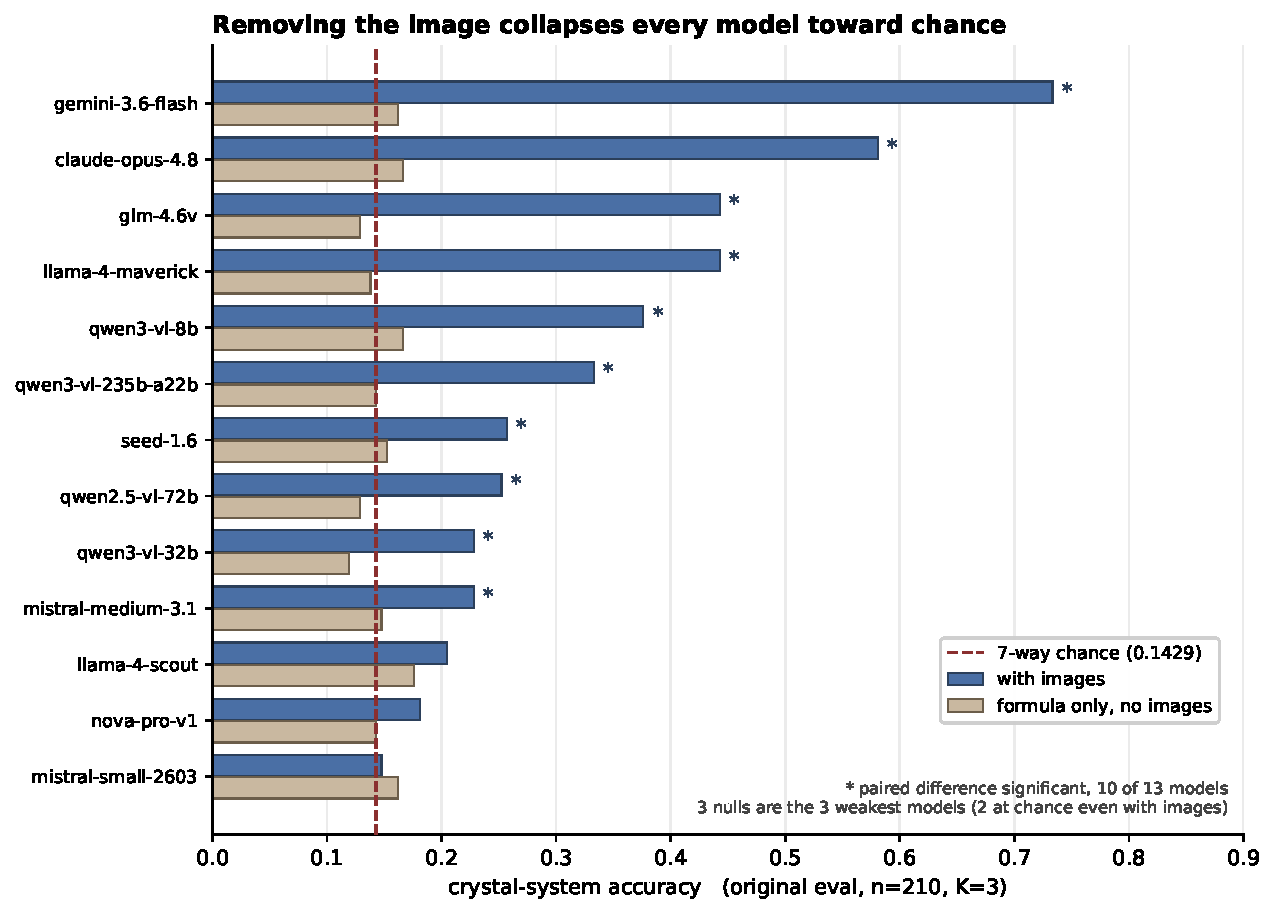
\includegraphics[width=0.8\linewidth]{figures/noimage.pdf}
\caption{Image-removal control: each model answered the identical prompt with the five renders and with the
chemical formula alone, paired per structure (original sample, $n=210$, $K=3$, 13 scored of 16 attempted).
Stars mark models whose paired difference is significant; the dashed line is seven-way chance.}
\label{fig:noimage}
\end{figure}

\textbf{A baseline comparison we previously reported does not survive scale-up, and we retire it.} On the
original sample every model falls below a shape-free baseline reading only atom count, density and cell
volume (0.4429 against 0.5286, one-sided $p = 0.0078$). We regenerated the evaluation set at $n = 1933$
under identical rules: same composition exclusion, verified zero overlap with training and both earlier
samples, stratified 285 per system before quarantine, with 62 structures (3.11\%) removed for label
instability under the tolerance sweep. On that sample the baseline falls to 0.2054. Because the new draw
also has larger cells (median 38 atoms against 14), we ran a size-matched control restricted to the
original's 95th percentile: the baseline is 0.2205 there, so the shift is not a cell-size artefact.
\emph{The 0.5286 was a property of the original draw, not of the task}, and the below-baseline claim is
scoped to that sample rather than asserted generally.

The same control shows the oracle's apparent drop at scale \emph{is} a cell-size effect: 0.8774 on the full
sample but 0.9459 at matched cell size, within 0.0065 of the original. More atoms per cell means more
projective coincidence and more correspondence ambiguity, which is the failure set of
Proposition~\ref{prop:ident}. The ceiling-to-model gap, which is what this paper rests on, therefore
survives scale-up (0.9459 against 0.4429), while the baseline comparison does not.

\textbf{Run-to-run spread is a benchmark property.} An unplanned second execution of the sweep gives a mean
absolute difference of 5.0 structures and a maximum of 11, so adjacent leaderboard rows are not separable
and the ordering is not exact.

Two axes are reported in full in the supplementary and summarised here, because both end by disclaiming
themselves and neither carries a main-text claim.

\textbf{Cue sufficiency.} Whether the conventional-cell metric alone determines the crystal system splits
the samples $140/70$ and $141/69$ and is a stable property of the render convention with no accuracy
mechanism attached: an earlier claim that pixel accuracy simply drops on the ambiguous stratum failed four
independent tests and is withdrawn. A contrast against a cell-metric control does widen on that stratum for
all three frontier models on both samples (Figure~\ref{fig:cuesuff}), but the stratum is $60/70$ and
$58/69$ hexagonal-or-trigonal, so the finding is close to a restatement of that one degeneracy, and the
degeneracy-removed residual rests on $n=10$ and $n=12$.

\textbf{One generation of model progress.} It does not erase the axis (Figure~\ref{fig:generational}): from
gemini-2.5-flash to gemini-3.6-flash the newer model gains more on the ambiguous stratum in raw terms but
closes less of its headroom to the oracle (54.1\% against 64.0\%), and one model pair is a comparison
rather than a trend.
